%!TEX ROOT=main.tex

Following pages include the outputs from the design stage of the LoRa module.

Due to the use of incompatible crystal oscillator in this version of the LoRa module a v0.2 was also designed. It includes the TCXO modification, as discussed in \ref{section:module-schematic}, an optimized pinout and some other minor edits. The v0.2 was not manufactured because the tuning of the front-end was not realized within the deadline of the project. 

The modifications needed for the v0.1 to function had little impact on the results and the additional resources that would need to be invested in manufacturing a second version with other possible defects, that could be resolved and tested on the v0.1, was not justified.


\begin{table}[H]
    \begin{center}
    \caption{\label{table:board-layers}Module board layer signal and power assignments}
        \begin{tabular}{|l|l|l|} \hline
Qty &	Reference(s) &	Value \\ \hline
    4   & C101, C203, C208, C214 & 4.7u \\ \hline
    13  & C102, C204, C206, C207, C209, C210, C216, C218, C220, C221, C307, C309, C401 & 100n \\ \hline
    2   & C201, C202 & DNP \\ \hline
    1   & C211 & 470n \\ \hline
    3   & C213, C215, C217 &	33p \\ \hline
    1   & C219	& 3.3p \\ \hline
    1   & C301	& GCM155R71E473KA55 \\ \hline
    1   & C302	& GCM1555C1H680JA16 \\ \hline
    1   & C303	& GRM0335C1H101GA01D \\ \hline
    2   & C304, C310	& GRM0335C1H390JA01D \\ \hline
    3   & C305, C311, C312	& DNP \\ \hline
    1   & D101	& B1861NB-05D000134U1930 \\ \hline
    1   & J101	& U.FL-R-SMT-1 \\ \hline
    1   & L201	& BK1608HS601-T \\ \hline
    1   & L202	& MLZ2012M150W \\ \hline
    1   & L301	& LQW15AN47NG00 \\ \hline
    1   & L302	& 0R \\ \hline
    1   & Q101	& PMN48XP \\ \hline
    1   & R101	& 1M \\ \hline
    1   & R102	& 100k \\ \hline
    3   & R103, R201, R202	& 10k \\ \hline
    2   & R301, R302	& 100R \\ \hline
    1   & U201	& STM32WLE5CCUx \\ \hline
    1   & U301	& BALFHB-WL-05D3 \\ \hline
    1   & U302	& BGS12SN6E6327XTSA1 \\ \hline
    1   & U401	& SST26VF080A \\ \hline
    1   & XTAL201 &	NX2016SA-32MHZ-EXS00A-CS11336 \\ \hline
\end{tabular}
\end{center}
\end{table}

\begin{figure}
    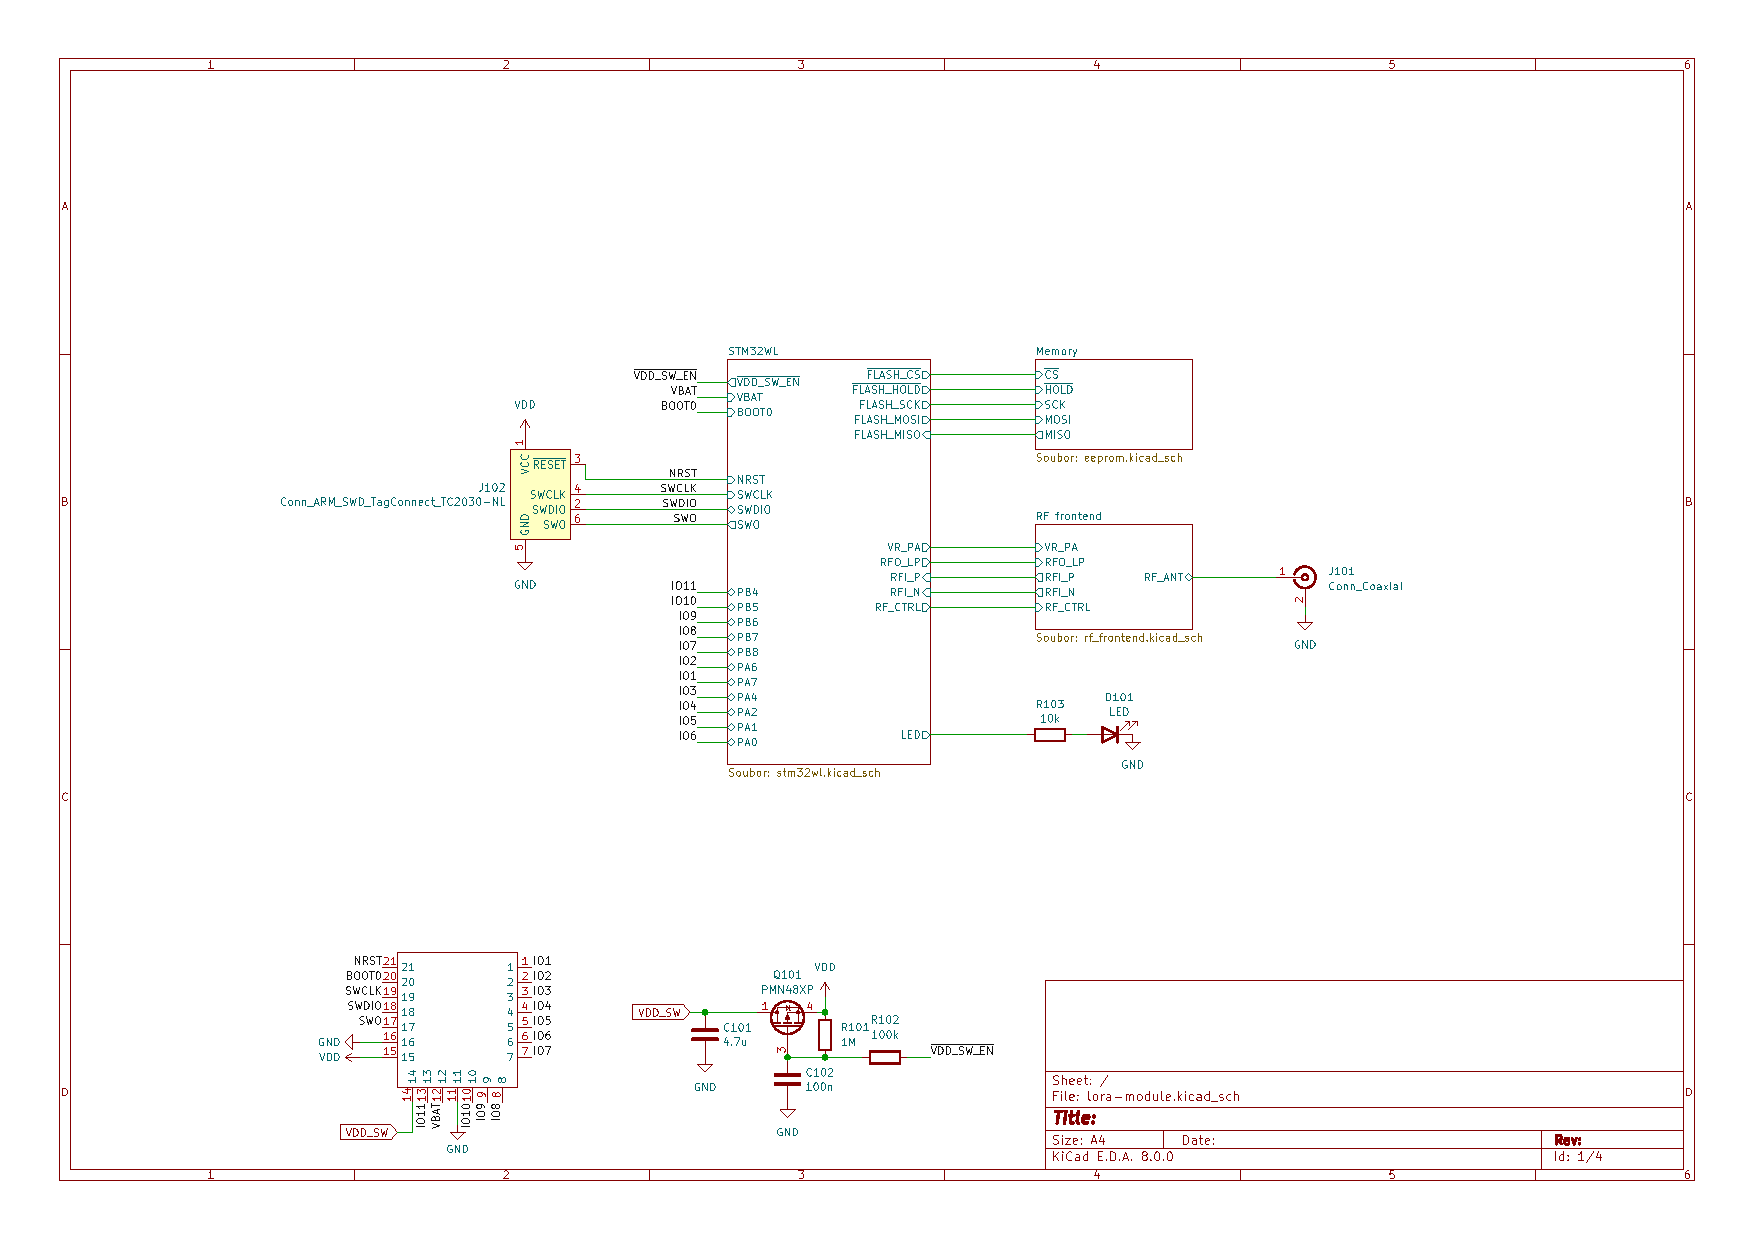
\includegraphics[page=1,angle=-90,width=\textwidth]{boards/v0.1/lora-module.pdf}
    \caption{\label{schematic:v0.1-1}Top level schematic sheet}
\end{figure}
\begin{figure}
    \includegraphics[page=2,angle=-90,width=\textwidth]{boards/v0.1/lora-module.pdf}
    \caption{\label{schematic:v0.1-2}STM32WLE5JC schematic sheet}
\end{figure}
\begin{figure}
    \includegraphics[page=3,angle=-90,width=\textwidth]{boards/v0.1/lora-module.pdf}
    \caption{\label{schematic:v0.1-3}RF frontend schematic sheet}
\end{figure}
\begin{figure}
    \includegraphics[page=4,angle=-90,width=\textwidth]{boards/v0.1/lora-module.pdf}
    \caption{\label{schematic:v0.1-4}Non-volatile memory schematic sheet}
\end{figure}

\begin{figure}
    \subfloat[Front layer]{\includesvg[width=.48\textwidth]{boards/v0.1/lora-module-F_Cu.svg}}\hfill
    \subfloat[Back layer]{\includesvg[width=.48\textwidth]{boards/v0.1/lora-module-B_Cu.svg}}\hfill
    \subfloat[Inner GND layer]{\includesvg[width=.48\textwidth]{boards/v0.1/lora-module-In1_Cu.svg}}\hfill
    \subfloat[Inner VCC layer]{\includesvg[width=.48\textwidth]{boards/v0.1/lora-module-In2_Cu.svg}}
    \caption{\label{board:v0.1}Module v0.1 PCB layer design}
\end{figure}

\begin{figure}
    \includesvg[width=\textwidth]{boards/v0.1/lora-module-F_Fab.svg}
    \caption{\label{board:v0.1-components}Module v0.1 component position reference}
\end{figure}
